\section{Enabling Software Fault Tolerance in MPI}
\label{sect:ompi}

% Issues that need to be fixed in ompi to enable just 
% error-return, don't explain how we use it yet, leave it for next 
% section

\subsection{Errors in MPI and On-Demand Checkpointing}

Contrary to all the proposed additions to the MPI standard introduced
in Section~\ref{sect:background}, we advocate in this paper that an
extremely efficient form of fault tolerance can be implemented, based
on the MPI standard, for those applications which can take advantage
of it. According to the paragraphs of the standard cited in the
previous section, when implementing a high-quality MPI library, the
application should regain control following a process failure.  This
control gives the application the opportunity to save
its state and exit gracefully, rather than the usual behavior of being
aborted by the MPI implementation itself. In most current MPI
implementations, MPI\_ERRORS\_ABORT is the default (and often, only
functional) MPI\_Errhandler.  However, the MPI standard also defines
another handler called MPI\_ERRORS\_RETURN. This handler
should perform any necessary cleanup at the library level and then
return to the application, giving it the opportunity to continue if
possible. The MPI standard does not require that any MPI function
calls continue to operate after an error is returned (thus after a
failure), but even without MPI calls, we will show that it is possible
for the application to complete its computation, or save enough
information after the failure is detected to allow for continuing the
computation in a new application.

\abft algorithms are capable of restoring missing data from redundant
information located in the other processes. This requires, of course,
to communicate between processes, and we acknowledge that requiring
from the MPI implementation to maintain functioning MPI calls after a
failure hit one of the nodes is too demanding in front of the current
standard. However, expecting that the living processes continue to
work after a failure, and to be able to access the other functionalities
of the system seems significantly less perturbing for the MPI
implementors. We will present in the second part of this section how
this was done in the \ompi implementation.

\begin{figure}
\begin{center}
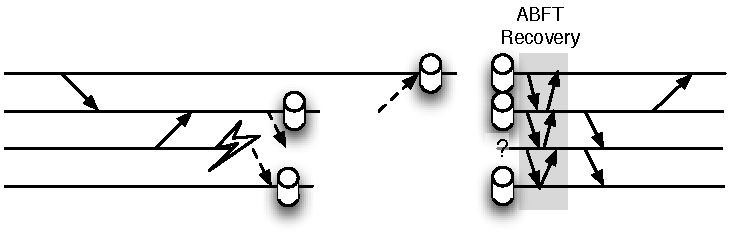
\includegraphics[width=.9\linewidth]{figures/idea.pdf}
\caption{Execution diagram of an On-Demand Checkpointing approach with
  one failure\label{fig:idea}}
\end{center}
\end{figure}

Under this assumption, consider the figure~\ref{fig:idea}. Horizontal
lines represent the execution of different processes in two successive
MPI applications. Living processes are allowed to call any other type
of operations that does not depend on MPI after a fatal error is
returned. In the proposed general approach, processes that detect a
failure will stop immediately to use MPI, save, on a file (local or
remote, depending on the machine capability), all necessary
information to proceed with the \abft algorithm and exit without
calling MPI\_Finalize. This operation does not require communication
if a filesystem, or any other way to do Input/Output operations remains
available. Because process exiting will be considered as failed from
the MPI perspective, all processes of the MPI application will
eventually discover the initial failure, and the application that was
hurt by a failure will then terminate. The user (or a controlling
script), that launched the MPI application in the first place, can
detect the failure by checking the return code of the MPI runtime
system.

Usually, the execution is terminated at this point. However, the user
or the script can launch a new MPI application on the same
resources. This new application will load the local states (second
series of lines in the figure), when available. If the file is not
available, it means that it was not saved for the requesting ranks,
and thus that these ranks were the ones hit by a failure in the
previous run. In the new MPI application, the MPI system is
functional. So, communications are enabled, and the recovery procedure
of the \abft approach can be called to restore the data of the
process(es) that did not find it locally. From this point on, the
application can continue its normal execution, as the global state has
been restored by the \abft recovery procedure. If another failure hits
the system again during the recovery, the local states are not
updated, and the relaunch starts from the beginning. If another
failure hits the system after the \abft recovery, the same procedure
is followed to handle it.

\subsection{On-Demand Checkpointing and Rollback Recovery}

An On-Demand Checkpointing application behaves similarly to the
familiar checkpoint/restart approach. However, by not periodically
saving a checkpoint to stable storage, the application gains an
enormous overhead reduction. Rather than needing to tune an optimal
checkpoint interval and periodically save that checkpoint to stable
storage, the application only needs to save the ``checkpoint'' once
after the failure has already occurred. This has the added benefit of
incurring zero checkpoint-related overhead in the fault-free case, a
consideration that is very important on reliable systems with a low
likelihood of failure.  This means that the same code can be run on
both reliable and non-reliable hardware without modification. This
method of on-demand checkpointing gives the user a safe place to write
its checkpoint before being aborted by the MPI library.

In traditional checkpointing, a complete set of checkpoints is saved
periodically. With on-demand checkpointing, the failed processes will
not write their checkpoints as they have already failed and will most
likely be unable to do so (although link failures could be taken into
consideration: in this case, all processes are able to save the local
state, and the recovery procedure will simply consist in determining
the global state at the moment of failure). Because of this, the
algorithm will need to be able to recover the failed process and
generate all necessary information to bring it back up to the same
point as the other non-failed processes.

There is another fundamental difference between On-Demand
Checkpointing and Coordinated Checkpointing, or most of the rollback
recovery approaches. In traditional rollback recovery, the checkpoint
images must be saved to a reliable media. It is, in particular,
critical to recover the checkpoint image of the failed process to
ensure the recovery. In \cite{HierarchicalCheckpoint09} it is proposed
to keep a local copy of the checkpoint image for the living processes,
if local storage is available, in order to reduce the I/O stress on
the remote storage system, but the failed process must have their
images stored remotely. Since the system does not know what processes
are going to fail at the time of checkpoint, all images must be also
stored remotely. Thus, the (distributed) checkpoint can be considered
complete only when all processes have stored their image on a resource
that has a low probability to fail simultaneously with them. 

In the case of On-Demand Checkpointing, the situation is completely
different: only the checkpoint image of the living processes at the
moment of failure is required. Thus, local storage can be considered
if the same resources can be reused for the restarted MPI
application. Similarly, traditional rollback recovery cannot rely on
local caching of the shared filesystem, while On-Demand Checkpointing
can use this operating system feature to accelerate significantly the
time it takes to save the checkpoint image, and reload it, if memory
is available.

The cost of the On-Demand Checkpointing approach is of course similar
to the cost of any \abft approach: the application might need to do
extra computation during the whole execution, to maintain internal
redundancy that will enable it to restore the missing data when a
failure hits any of the nodes. However, \abft techniques often have an
excellent scalability. For example, the \abft QR operation that we use
to illustrate On-Demand Checkpointing in this work has an overhead on
the fault-free execution inverse proportional to the number of
participating processes, and therefore nodes.
% that decreases when the number of nodes increases.

% Implementation details, might go to a separate section before 
% experiments though, we have room, that would better separate concept 
% from details. 

\subsection{\ompi Implementation\label{sec:mpi}}

\ompi is an MPI 2.2 implementation architected such that it contains
two main levels, the runtime (ORTE) and the MPI implementation (OMPI),
with an additional level to provide support to the other two
(OPAL). As with most MPI library implementations, the default behavior
of \ompi is to abort after a process failure. This policy was
implemented in the runtime system, preventing any kind of decision
from the MPI layer, or the user-level. The major change implemented
for this work was to make the runtime system resilient, and leave the
policy decision in case of failure to the MPI library, and ultimately
to the user application. To do so, we included an incarnation number
in the process names, as they are known by the runtime
system. Incarnation numbers are used to count how many times a process
has failed and are necessary to track the status of all of the
processes in order to know which processes are alive, which have
failed, and reconcile contradictory views. Once the incarnation numbers
are included in the runtime layer, the runtime error manager needs to
change its default behavior during a failure. Rather than notifying
the head node process (HNP) and starting an abort, we introduced a
notification phase, where all runtime processes are notified of the
failure so they can propagate this information to the MPI layer which
appropriately handles the failure according to the application's
instructions.

The runtime layer provides an out-of-band communication mechanism
(OOB) that relays messages through a routing policy implemented in the
routed component. This OOB layer is used to detect failures at the
runtime level, and propagate the failures notifications. We have
changed the routing algorithms to allow for a more dynamic network,
were processes of the OOB can leave the network due to a failure. The
underlying routing algorithm also has a significant influence on the
time it takes to detect a failure and notify all MPI processes, as the
experiments will show.

Like the runtime layer, the OMPI layer has a default behavior during a
process failure of calling MPI\_Abort. The alternative error handler
MPI\_ERRORS\_RETURN is made functional by receiving the failure
notification from the runtime system. When the case happens, all
outstanding communication requests involving the communicator with the
failed process are cancelled. This prevents any outstanding
communications with the failed process from causing a dependency issue
with future communications and ensures that the application will be
notified of the process failure when the MPI function that it is
calling returns a non-MPI\_SUCCESS error code.

In addition to allowing the application to select the MPI\_Errhandler
MPI\_ERRORS\_RETURN, the application can choose to implement custom
MPI\_Errhandlers, another feature of the current MPI standard. In
these custom MPI\_Errhandlers, the application can immediately perform
any post-failure operations, such as saving the local state. These
custom MPI\_Errhandlers provide enormous flexibility to the user.
